\documentclass[11pt]{article}
\usepackage{geometry}
\geometry{margin=1in}
\usepackage{amsmath,amssymb}
\usepackage{booktabs}
\usepackage{graphicx}
\usepackage{hyperref}
\usepackage{parskip}

\title{The Copy-Forward Pathway: A Fourth Axis of the Adaptive Window\\
       in Viability-Constrained Memory Systems}
\author{VCSM Theory Series --- Paper 12}
\date{}

\begin{document}
\maketitle

\begin{abstract}
Papers 10--11 identified two boundaries governing the adaptive window of the
Viability-Constrained Coupled Map Lattice (VCML): a lower bound $\nu_{\rm cryst}$
set by field decay, and an upper bound $\nu_{\rm max}$ set by consolidation
access. Here we isolate a third structural maintenance pathway --- copy-forward
inheritance --- which operates independently of both consolidation and decay.
At birth, each new site inherits a blend of local noise and its neighbor's
\texttt{fieldM}: $h_{\rm new} = (1-\beta_s)\,\varepsilon + \beta_s F_j$, with
$\beta_s$ (\texttt{SEED\_BETA}) controlling inheritance strength. We show that
(i)~ablating copy-forward ($\beta_s=0$) has minimal impact at low $\nu$ where
consolidation dominates, but (ii)~strong copy-forward ($\beta_s=0.50$) shifts
$\nu^*$ by 4$\times$ into the mid-turnover regime. A product-collapse test
($\nu \times \beta_s = \text{const}$) fails: iso-product pairs vary in sg4 by
up to $24\times$, because field quality $F_{\rm eq}$ itself degrades with $\nu$.
We conclude that the adaptive regime is governed by at least four
independent parameters $\{\nu,\,\nu_{\rm cryst},\,\nu_{\rm max}^{\rm consol},\,
\beta_s\}$ forming a viability volume in control space, not a single scalar law.
This result motivates the 4D framing developed in Paper~13.
\end{abstract}

%----------------------------------------------------------------------
\section{Background and Motivation}
%----------------------------------------------------------------------

The VCSM learning rule (Papers 0--6) maintains spatial structure in a lattice
of cells with mandatory turnover. Papers~8--11 progressively isolated the
scalar parameters governing the \emph{adaptive window} $[\nu_{\rm cryst},\,
\nu_{\rm max}]$ of turnover rates $\nu$ at which spatial differentiation
(sg4) peaks:

\begin{align}
\nu_{\rm cryst} &= \frac{|\ln(\text{FIELD\_DECAY})|}{\ln 2}
   &&\text{(lower bound: memory crystallizes below this)} \label{eq:nu_cryst}\\
\nu_{\rm max}^{\rm consol} &\approx P_{\rm calm} \cdot \alpha_F \cdot
   \text{FIELD\_DECAY}^{1/\nu}
   &&\text{(upper bound: consolidation cannot keep up above this)} \label{eq:nu_max}
\end{align}

However, three anomalies persisted across Papers~10--11: structure maintained
at (i)~$\text{WR}=7.2$ where $P_{\rm calm}\approx 0.001$, (ii)~$\text{SS}=40$
where $\nu_{\rm max}^{\rm consol} < \nu_{\rm cryst}$, and (iii)~$\alpha_F=0.04$
where the window was predicted to vanish. All three share a common candidate:
the \emph{copy-forward pathway}, in which cell births propagate existing field
structure without requiring calm consolidation.

This paper directly tests the copy-forward pathway by sweeping \texttt{SEED\_BETA}
($\beta_s$) from 0 (full ablation) to 0.50 (strong inheritance), and by
testing whether the product $\nu \times \beta_s$ collapses the data as a
simple rate model would predict.

%----------------------------------------------------------------------
\section{Methods}
%----------------------------------------------------------------------

\subsection{Experiment 1: SEED\_BETA Sweep}

We hold all parameters at reference values (WR$=4.8$, WD$=15$, SS$=10$,
FIELD\_DECAY$=0.9997$, $\alpha_F=0.16$, $\kappa=0.020$) and vary $\beta_s
\in \{0.00,\,0.05,\,0.10,\,0.25,\,0.50\}$ across the full 12-point $\nu$
grid (5 seeds per condition, 300 total runs).

At birth, the dead site's hidden state is reinitialized as:
\[
h_{\rm new} = (1-\beta_s)\,\mathcal{N}(0,\,0.1) + \beta_s\,F_j
\]
where $j$ is a random live neighbor. When $\beta_s=0$, births inject pure
noise; copy-forward is fully ablated.

\subsection{Experiment 2: Product Collapse Test}

We run a $4\times4$ grid: $\nu \in \{0.001,\,0.002,\,0.005,\,0.010\}$ by
$\beta_s \in \{0.05,\,0.10,\,0.25,\,0.50\}$ (5 seeds, 80 total runs). If
copy-forward rate $\Gamma_{\rm cf} = \nu \times \beta_s \times F_{\rm eq}$
with $F_{\rm eq}$ independent of $\nu$, iso-product pairs
$(\nu_1,\,\beta_{s,1})$, $(\nu_2,\,\beta_{s,2})$ with
$\nu_1\beta_{s,1} = \nu_2\beta_{s,2}$ should yield equal sg4.

%----------------------------------------------------------------------
\section{Results}
%----------------------------------------------------------------------

\subsection{Experiment 1: Copy-Forward Has Regime-Dependent Impact}

\begin{table}[h]
\centering
\caption{SEED\_BETA sweep results. Columns show sg4 at each $\nu$ value.
$\nu_{\rm cryst}=4.3\times10^{-4}$ fixed throughout.}
\label{tab:exp1}
\small
\begin{tabular}{ccc|rrrrrr}
\toprule
$\beta_s$ & $\nu^*$ & sg4* &
  \multicolumn{6}{c}{sg4 profile at selected $\nu$} \\
& & &
  $10^{-4}$ & $5{\times}10^{-4}$ & $10^{-3}$ & $2{\times}10^{-3}$ &
  $5{\times}10^{-3}$ & $10^{-2}$ \\
\midrule
0.00 & 0.0005 & 394 & 210 & 394 & 311 & 215 & 113 &  60 \\
0.05 & 0.0005 & 402 & 212 & 402 & 324 & 233 & 121 &  64 \\
0.10 & 0.0005 & 408 & 215 & 408 & 337 & 254 & 130 &  67 \\
0.25 & 0.0005 & 419 & 223 & 419 & 376 & 328 & 161 &  80 \\
0.50 & 0.0020 & 500 & 246 & 407 & 443 & 500 & 218 & 107 \\
\bottomrule
\end{tabular}
\end{table}

Three key observations from Table~\ref{tab:exp1}:

\textbf{(1) Ablation at low $\nu$ is weak.} At $\nu=5\times10^{-4}$, sg4 changes
from 394 ($\beta_s=0$) to 419 ($\beta_s=0.25$), a 6\% increase. The
consolidation pathway alone ($\beta_s=0$) is nearly sufficient at low turnover.
This confirms that copy-forward is not the primary mechanism in the frozen
regime: long-lived sites consolidate via the standard VCSM pathway.

\textbf{(2) Copy-forward dominates at moderate $\nu$.} At $\nu=0.002$, sg4
rises from 215 ($\beta_s=0$) to 500 ($\beta_s=0.50$), a 133\% increase.
At this turnover rate, consolidation is limited by calm-streak timing ($P_{\rm
calm}\approx0.015$), but copy-forward births propagate field structure without
requiring calm periods.

\textbf{(3) Strong copy-forward shifts $\nu^*$.} At $\beta_s=0.50$, the
optimal turnover rate shifts from $\nu^*=5\times10^{-4}$ to $\nu^*=0.002$,
a 4$\times$ displacement. The copy-forward pathway effectively raises
$\nu_{\rm max}$ by extending structural maintenance into the high-turnover
regime.

\subsection{Experiment 2: Product Hypothesis Fails; F\_quality is $\nu$-Dependent}

\begin{table}[h]
\centering
\caption{sg4 heatmap from the $\nu \times \beta_s$ grid. Products $\nu\beta_s$
are shown in parentheses. Iso-product pairs at $\nu\beta_s=5\times10^{-4}$
(diagonal entries) vary from 19 to 443 --- a $24\times$ range.}
\label{tab:exp2_sg4}
\small
\begin{tabular}{c|cccc}
\toprule
$\nu \backslash \beta_s$ & 0.05 & 0.10 & 0.25 & 0.50 \\
\midrule
0.001 & 324 $(5{\times}10^{-5})$
      & 337 $(10^{-4})$
      & 376 $(2.5{\times}10^{-4})$
      & 443 $(\mathbf{5{\times}10^{-4}})$ \\
0.002 & 233 $(10^{-4})$
      & 254 $(2{\times}10^{-4})$
      & 328 $(\mathbf{5{\times}10^{-4}})$
      & 500 $(10^{-3})$ \\
0.005 &  64 $(2.5{\times}10^{-4})$
      &  67 $(\mathbf{5{\times}10^{-4}})$
      &  80 $(1.25{\times}10^{-3})$
      & 107 $(2.5{\times}10^{-3})$ \\
0.010 &  19 $(\mathbf{5{\times}10^{-4}})$
      &  20 $(10^{-3})$
      &  24 $(2.5{\times}10^{-3})$
      &  39 $(5{\times}10^{-3})$ \\
\bottomrule
\end{tabular}
\end{table}

Table~\ref{tab:exp2_sg4} shows the iso-product failure. The four
\textbf{bold} entries all share $\nu\beta_s = 5\times10^{-4}$ but produce
sg4 values of 443, 328, 67, and 19. The product hypothesis requires these
to be equal; instead they span a $24\times$ range.

The explanation is immediate from the field-norm proxy $\bar{F}$ (mean
$\|F_i\|$ at end of run):

\begin{table}[h]
\centering
\caption{Mean field norm $\bar{F}$ (proxy for $F_{\rm quality}$) across the
$\nu \times \beta_s$ grid. $\bar{F}$ decays faster than $1/\nu$ as $\nu$
increases, invalidating the constant-$F_{\rm quality}$ assumption.}
\label{tab:exp2_fnorm}
\small
\begin{tabular}{c|cccc}
\toprule
$\nu \backslash \beta_s$ & 0.05 & 0.10 & 0.25 & 0.50 \\
\midrule
0.001 & 502 & 523 & 596 & 753 \\
0.002 & 318 & 335 & 400 & 542 \\
0.005 &  89 &  92 & 103 & 128 \\
0.010 &  29 &  30 &  34 &  46 \\
\bottomrule
\end{tabular}
\end{table}

From $\nu=0.001$ to $\nu=0.010$ (10$\times$), $\bar{F}$ at $\beta_s=0.25$
drops from 596 to 34 (17.5$\times$). Field quality therefore degrades
\emph{faster} than $1/\nu$. The copy-forward rate:
\[
\Gamma_{\rm cf} = \nu \times \beta_s \times F_{\rm quality}(\nu)
\]
is not a simple product because $F_{\rm quality}$ is itself a declining
function of $\nu$. As $\nu$ increases, the shorter site lifetimes suppress
consolidation, eroding the field before births can relay it. This creates a
feedback loop: higher $\nu$ lowers $F_{\rm quality}$, which weakens
copy-forward, which further reduces $F_{\rm quality}$.

\subsection{Two Regimes of Structural Maintenance}

Together, Experiments~1 and~2 resolve the copy-forward pathway's role:

\begin{itemize}
\item \textbf{Low $\nu$ ($\nu \lesssim 5\times10^{-4}$)}: Long site lifetimes
allow consolidation to build high $F_{\rm quality}$. Copy-forward is
irrelevant because births are rare. $\nu^*$ and sg4 are nearly identical
whether $\beta_s=0$ or $\beta_s=0.25$.

\item \textbf{Moderate $\nu$ ($5\times10^{-4} < \nu \lesssim 0.005$)}: Sites
die faster than the calm-streak gate allows consolidation. Copy-forward
becomes the dominant maintenance pathway: each birth reinjects neighbor
field structure. $\beta_s$ now strongly controls both sg4 height and $\nu^*$.

\item \textbf{High $\nu$ ($\nu > 0.005$)}: Even copy-forward fails.
Field quality $F_{\rm quality} \to 0$ because consolidation cannot keep up
at all. Structure collapses regardless of $\beta_s$.
\end{itemize}

This defines \emph{three turnover regimes} rather than two (frozen/adaptive):
consolidation-dominated, copy-forward-dominated, and collapsed. The adaptive
window of prior papers corresponds to the union of the first two regimes.

%----------------------------------------------------------------------
\section{Discussion}
%----------------------------------------------------------------------

\subsection{The Control Space is Four-Dimensional}

Papers~8--12 have now identified four independent axes of the adaptive window:

\begin{enumerate}
\item \textbf{Turnover} $\nu$: the external control parameter.
\item \textbf{Memory decay} (FIELD\_DECAY $\to \nu_{\rm cryst}$): sets lower
    boundary independently of all other parameters.
\item \textbf{Consolidation access} (SS, $\alpha_F$, WR/WD $\to P_{\rm calm}$,
    $\nu_{\rm max}^{\rm consol}$): sets upper consolidation boundary.
\item \textbf{Copy-forward} ($\beta_s \to \nu_{\rm max}^{\rm cf}$): extends
    the upper boundary into the moderate-turnover regime, independently of
    $P_{\rm calm}$.
\end{enumerate}

These four axes are mutually irreducible: no two-dimensional scalar
($\Xi$, $\Psi$, or product $\nu\beta_s$) collapses the data across all experiments.
The adaptive regime is better described as a \emph{viability volume} in
this four-dimensional control space:
\[
\mathcal{V} = \bigl\{\,(\nu,\,\text{FD},\,P_{\rm calm}\cdot\alpha_F,\,\beta_s)
: \nu_{\rm cryst} < \nu
< \max(\nu_{\rm max}^{\rm consol},\,\nu_{\rm max}^{\rm cf})
\,\bigr\}
\]

The prior series of partial scalars were projections of this volume onto
two-dimensional slices:
$\Xi$ captured the consolidation face (Papers~8--9);
$\Psi$ captured the consolidation--decay trade-off (Paper~10);
the substrate constants paper (Paper~11) located the volume boundaries;
this paper (Paper~12) maps the copy-forward face.

\subsection{Why the 2D Attempts Partly Worked}

Each 2D projection succeeded within its constrained parameter range and
failed at the boundaries:
\begin{itemize}
\item $\Psi$ predicted the window for weak $\beta_s$ (low copy-forward contribution)
  but failed at high WR and extreme SS (where copy-forward anomalies dominated).
\item The SS sweep (Paper~11) predicted window collapse at SS$=40$ but found
  persistent structure; copy-forward maintained sg4=45 even with $P_{\rm
  calm} \approx 10^{-4}$.
\end{itemize}
These are not failures of the parameter sweep design; they are geometrically
necessary consequences of projecting a 4D object onto a 2D face.

\subsection{Implications for Paper 13}

The appropriate goal for Paper~13 is not a single universal scalar but
a characterization of the minimal state space sufficient to predict
$\nu^*$ and sg4$^*$. We propose to test whether a 4D inequality system:
\[
\nu > \nu_{\rm cryst}(\text{FD}),\qquad
\nu < \nu_{\rm max}^{\rm consol}(P_{\rm calm},\,\alpha_F)
    + \nu_{\rm max}^{\rm cf}(\beta_s,\,F_{\rm quality}(\nu))
\]
with $\nu^* \approx \sqrt{\nu_{\rm cryst} \cdot \nu_{\rm max}^{\rm total}}$
as the geometric mean, suffices to predict $\nu^*$ across the full
parameter range of Papers~8--12.

%----------------------------------------------------------------------
\section{Conclusion}
%----------------------------------------------------------------------

The copy-forward pathway ($\beta_s > 0$) is a fourth independent axis of the
adaptive window. It is redundant with consolidation at low $\nu$ but becomes
the primary structural maintenance mechanism at moderate turnover. The simple
product $\nu\beta_s$ does not collapse the data because field quality
$F_{\rm quality}$ degrades nonlinearly with $\nu$, creating a feedback loop.
The adaptive regime of VCML is governed by a four-dimensional viability
volume, not a single scalar, and each paper in this series has mapped one
face of that object. Paper~13 characterizes the complete volume.

\begin{figure}[p]
\centering
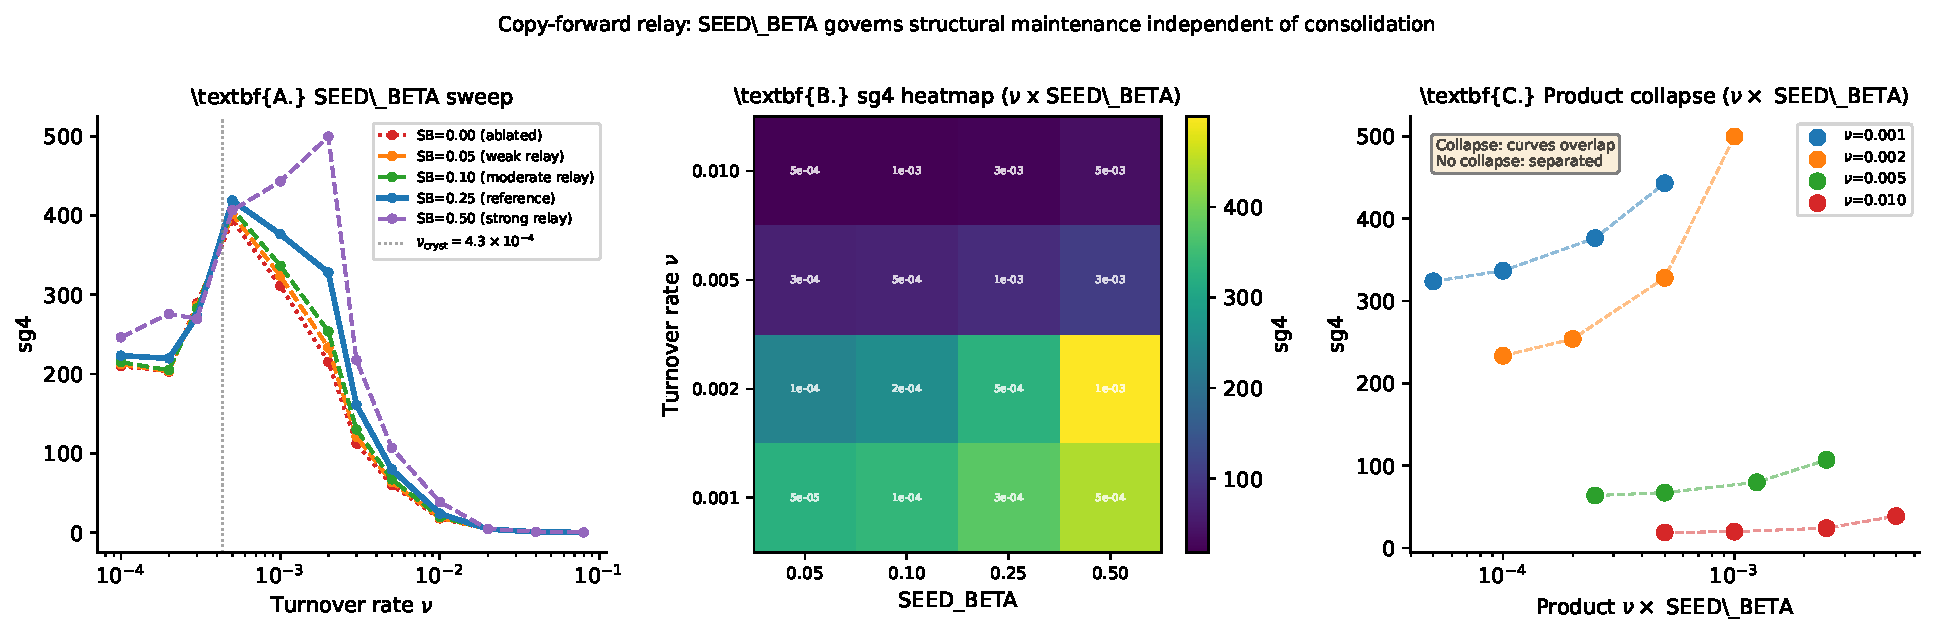
\includegraphics[width=\linewidth]{paper12_figure1.pdf}
\caption{
\textbf{A.}~SEED\_BETA sweep across the full $\nu$ range. At low $\nu$ the
profiles are nearly identical (consolidation dominates); at $\nu=0.002$,
sg4 doubles from $\beta_s=0$ to $\beta_s=0.50$. Strong copy-forward
($\beta_s=0.50$) shifts $\nu^*$ from $5\times10^{-4}$ to $2\times10^{-3}$.
\textbf{B.}~sg4 heatmap over the $\nu\times\beta_s$ grid. Diagonals
correspond to iso-product pairs; their large variation in sg4 falsifies the
product hypothesis. Products (italicized values) span the same range but
sg4 varies 24$\times$.
\textbf{C.}~Scatter of sg4 vs.\ $\nu\beta_s$ colored by $\nu$. Separated
curves confirm that $\nu$ and $\beta_s$ have independent effects beyond
their product.
}
\label{fig:fig1}
\end{figure}

\end{document}
